% ============================================================
% 第14章：函数在一点处的极限——ε-δ 定义
% ============================================================

\chapter{函数在一点处的极限——ε-δ 定义}

\begin{applicationbox}
\textbf{学完本章你能做什么？}
\begin{enumerate}
  \item 理解函数在一点处极限的 \textbf{ε-δ 定义}
  \item 掌握左右极限的概念——从左侧和右侧趋近
  \item 用 ε-δ 证明简单的函数极限
\end{enumerate}
\end{applicationbox}


% ============================================================
\section{从 \(x \to \infty\) 到 \(x \to a\)}
% ============================================================

第13章我们学了 \(x \to \infty\) 时的极限——函数在无穷远处的行为。

现在问一个更基本的问题：当 \(x\) 趋近于一个\textbf{有限数 \(a\)} 时，\(f(x)\) 会怎样？

\[
\lim_{x \to a} f(x) = L
\]

\textbf{含义：} 当 \(x\) 越来越接近 \(a\)（但不等于 \(a\)）时，\(f(x)\) 越来越接近 \(L\)。

\begin{examplebox}[1——直观例子]
\[
f(x) = 2x + 1,\quad \lim_{x \to 2} f(x) = 5
\]

验证：
\[
x=1.9 \to f=4.8,\; x=1.99 \to f=4.98,\; x=1.999 \to f=4.998
\]
\[
x=2.1 \to f=5.2,\; x=2.01 \to f=5.02,\; x=2.001 \to f=5.002
\]

不管从左边还是右边靠近 2，\(f(x)\) 都靠近 5。
\end{examplebox}


% ============================================================
\section{ε-δ 定义}
% ============================================================

\begin{definitionbox}[函数极限的 ε-δ 定义]
设 \(f(x)\) 在 \(x=a\) 的某个去心邻域内有定义。
如果对\textbf{任意} \(\varepsilon > 0\)，都\textbf{存在} \(\delta > 0\)，
使得当 \(0 < |x - a| < \delta\) 时，有
\[
|f(x) - L| < \varepsilon
\]
则称 \(\displaystyle \lim_{x \to a} f(x) = L\)。
\end{definitionbox}

\begin{examplebox}[2——ε-δ 的几何意义]
\begin{center}
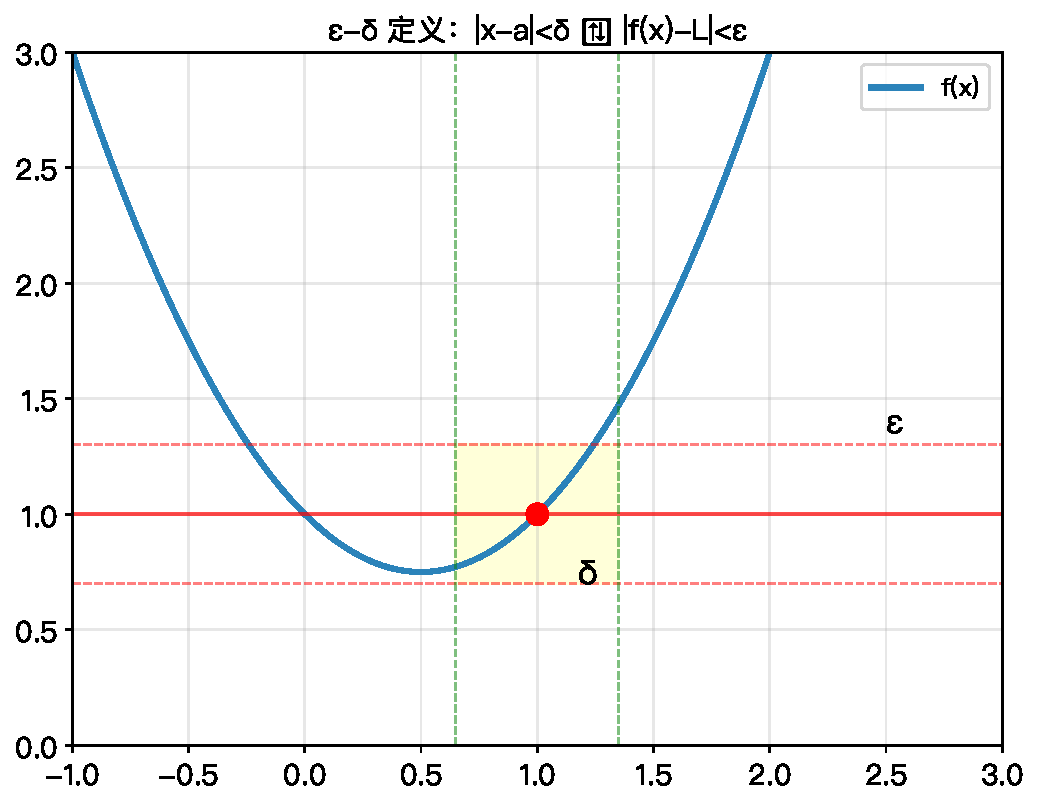
\includegraphics[width=0.7\textwidth]{figures/ch14_epsilon_delta.pdf}
\end{center}

\textbf{解读：}
\begin{itemize}
  \item 给你一个 \(\varepsilon\)（对 \(y\) 方向的精度要求）
  \item 我找到一个 \(\delta\)（\(x\) 方向的范围）
  \item 只要 \(x\) 在 \(a\) 的 \(\delta\) 邻域内（但不等于 \(a\)）
  \item \(f(x)\) 就一定在 \(L\) 的 \(\varepsilon\) 邻域内
\end{itemize}
\end{examplebox}


% ============================================================
\section{左右极限}
% ============================================================

\begin{definitionbox}[左右极限]
\begin{itemize}
  \item \textbf{左极限}：\(x\) 从左侧趋近 \(a\)（\(x \to a^-\)），记 \(\displaystyle \lim_{x \to a^-} f(x)\)
  \item \textbf{右极限}：\(x\) 从右侧趋近 \(a\)（\(x \to a^+\)），记 \(\displaystyle \lim_{x \to a^+} f(x)\)
\end{itemize}

极限存在的\textbf{充要条件}：左右极限都存在且相等。
\end{definitionbox}

\begin{examplebox}[3——左右极限不相等]
\[
f(x) = 
\begin{cases}
x + 1, & x \ge 0 \\
x - 1, & x < 0
\end{cases}
\]

\[
\lim_{x \to 0^+} f(x) = 1,\qquad
\lim_{x \to 0^-} f(x) = -1
\]

左右极限不相等 \(\Rightarrow\) \(\displaystyle\lim_{x \to 0} f(x)\) 不存在。
\end{examplebox}


% ============================================================
\section{本章小结}
% ============================================================

\begin{progressbox}
\textbf{ε-δ 定义}：\(\forall\varepsilon>0,\exists\delta>0\) 使 \(0<|x-a|<\delta \Rightarrow |f(x)-L|<\varepsilon\)

\textbf{左右极限}：\(x \to a^-\)（左）和 \(x \to a^+\)（右）\\
极限存在 \(\iff\) 左右极限存在且相等
\end{progressbox}

% ============================================================
% 习题
% ============================================================
\section{习题}

\begin{exercise}[0]
求 \(\displaystyle\lim_{x\to 1} (2x+1)\)。
\end{exercise}
\begin{exercise}[0]
判断：\(\displaystyle\lim_{x\to 0} \frac{|x|}{x}\) 存在吗？
\end{exercise}
\begin{exercise}[0]
若左右极限不相等，极限存在吗？
\end{exercise}
\begin{exercise}[0]
\(\varepsilon\)-\(\delta\) 定义中，\(\varepsilon\) 和 \(\delta\) 哪个先给？
\end{exercise}

\begin{exercise}[1]
求 \(\displaystyle\lim_{x\to 3} (x^2-1)\)。
\end{exercise}
\begin{exercise}[1]
求 \(\displaystyle\lim_{x\to 0^-} \frac{1}{x}\)。
\end{exercise}
\begin{exercise}[1]
求 \(\displaystyle\lim_{x\to 0^+} \frac{1}{x}\)。
\end{exercise}
\begin{exercise}[1]
判断：\(\displaystyle\lim_{x\to 0} \frac{1}{x}\) 存在吗？
\end{exercise}

\begin{exercise}[2]
已知 \(f(x)=\frac{x^2-1}{x-1}\)（\(x\neq1\)），求 \(\lim_{x\to 1} f(x)\)。
\end{exercise}
\begin{exercise}[2]
求 \(\displaystyle\lim_{x\to 2} \frac{x^2-4}{x-2}\)。
\end{exercise}
\begin{exercise}[2]
设 \(f(x)=\begin{cases}x^2,&x\ge1\\2x-1,&x<1\end{cases}\)，求左右极限和极限。
\end{exercise}
\begin{exercise}[2]
用 ε-δ 语言写出 \(\lim_{x\to 2} (3x-1)=5\) 的证明框架。
\end{exercise}

\begin{exercise}[3]
计算 \(\displaystyle\lim_{x\to 0} \frac{\sin x}{x}\)（查计算器取 \(x=0.1,0.01,0.001\)）。
\end{exercise}
\begin{exercise}[3]
求 \(\displaystyle\lim_{x\to 4} \frac{\sqrt{x}-2}{x-4}\)。
\end{exercise}
\begin{exercise}[3]
已知 \(\lim_{x\to a} f(x)=L\)，用 ε-δ 语言证明 \(\lim_{x\to a} cf(x)=cL\)。
\end{exercise}
\begin{exercise}[3]
讨论 \(\displaystyle\lim_{x\to 0} \frac{1}{x^2}\) 是否存在。
\end{exercise}
\begin{exercise}[3]
若 \(\lim_{x\to a} f(x)=L\)，\(\lim_{x\to a} g(x)=M\)，证明 \(\lim_{x\to a} [f(x)+g(x)]=L+M\)。
\end{exercise}

\begin{exercise}[4]
用 ε-δ 语言证明 \(\displaystyle\lim_{x\to 2} (x^2-3x+1)=-1\)。
\end{exercise}
\begin{exercise}[4]
讨论 \(\displaystyle\lim_{x\to 0} \frac{1}{x}\sin\frac{1}{x}\) 是否存在。
\end{exercise}
\begin{exercise}[4]
证明：若 \(\lim_{x\to a} f(x)=L>0\)，则存在 \(\delta>0\) 使 \(0<|x-a|<\delta\) 时 \(f(x)>0\)。
\end{exercise}
\begin{exercise}[4]
求 \(\displaystyle\lim_{x\to 0} \frac{\tan x}{x}\)。
\end{exercise}
\begin{exercise}[4]
设 \(f(x)=\begin{cases}x\sin\frac1x,&x\neq0\\0,&x=0\end{cases}\)，讨论 \(\lim_{x\to0} f(x)\)。
\end{exercise}

\begin{exercise}[5]
用 ε-δ 语言证明 \(\displaystyle\lim_{x\to 1} \frac{1}{x}=1\)。
\end{exercise}
\begin{exercise}[5]
证明：若 \(\lim_{x\to a} f(x)=L\)，则 \(\lim_{x\to a} |f(x)|=|L|\)。
\end{exercise}
\begin{exercise}[5]
求 \(\displaystyle\lim_{x\to 0} \frac{\sqrt{1+x}-1}{x}\)。
\end{exercise}
\begin{exercise}[5]
求 \(\displaystyle\lim_{x\to 0} \frac{e^x-1}{x}\)。
\end{exercise}

\begin{exercise}[6]
用 ε-δ 语言证明 \(\displaystyle\lim_{x\to a} x^2=a^2\)。
\end{exercise}
\begin{exercise}[6]
证明极限的唯一性：若 \(\lim_{x\to a} f(x)=L\) 且 \(\lim_{x\to a} f(x)=M\)，则 \(L=M\)。
\end{exercise}
\begin{exercise}[6]
求 \(\displaystyle\lim_{x\to 0} \frac{\ln(1+x)}{x}\)。
\end{exercise}

\begin{exercise}[7]
用 ε-δ 语言证明：若 \(\lim_{x\to a} f(x)=L\)，\(\lim_{x\to a} g(x)=M\)，
则 \(\lim_{x\to a} f(x)g(x)=LM\)。
\end{exercise}

